\subsubsection{feature::forward\_list::ForwardListView}

\label{feature::forward_list::ForwardListView}
\begin{figure}[ht]
	\centering
	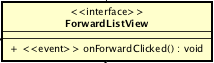
\includegraphics[scale=0.5]{Sezioni/SottosezioniST/img/app/ForwardListView.png}
	\caption{feature::forward\_list::ForwardListView}
\end{figure}

\begin{itemize}
\item \textbf{Descrizione}: Questa interfaccia rappresenta la view relativa all'inoltro di una lista-spesa.
\item \textbf{Utilizzo}: L'interfaccia viene utilizzata per disaccoppiare presenter e implementazione dell'inoltro, visualizza i dati che gli vengono passati dal presenter.
\item \textbf{Attributi}: 
\item \textbf{Metodi}:
\item \textbf{Eventi}:
\begin{itemize}
\item \textit{public onForwardClicked():void}\\
	Evento che rappresenta il click, da parte dell'utente, sull'oggetto visuale necessario all'inoltro di una lista-spesa.
\end{itemize}
\end{itemize}

\subsubsection{feature::forward\_list::view::ForwardListViewImpl}

\label{feature::forward_list::view::ForwardListViewImpl}
\begin{figure}[ht]
	\centering
	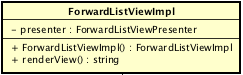
\includegraphics[scale=0.5]{Sezioni/SottosezioniST/img/app/ForwardListViewImpl.png}
	\caption{feature::forward\_list::view::ForwardListViewImpl}
\end{figure}

\begin{itemize}
\item \textbf{Descrizione}: Questa classe la componente grafica per l'inoltro di una lista-spesa, implementando l'interfaccia ForwardListView.
\item \textbf{Utilizzo}: Questa classe viene utilizzata dall'utente ogniqualvolta vuole inoltrare una lista-spesa.
\item \textbf{Attributi}:
\begin{itemize}
\item \textbf{private presenter:ForwardListViewPresenter}\\
Il presenter associato all'inoltro di una lista, al quale questa classe delega la gestione del comportamento dell'elemento di inoltro della lista.
\end{itemize}
\item \textbf{Metodi}: 
	\begin{itemize}
	\item \textit{public ForwardListViewImpl():ForwardListViewImpl}\\
	Il costruttore della classe ForwardListViewImpl.
	\item \textit{public renderView():string}\\
		Genera il codice HTML CSS JS necessario per visualizzare la componente grafica della lista-spesa necessaria all'inoltro di essa.
	\end{itemize}
\item \textbf{Eventi}:
\end{itemize}

\subsubsection{feature::forward\_list::presenter::ForwardListViewPresenter}

\label{feature::forward_list::presenter::ForwardListViewPresenter}
\begin{figure}[ht]
	\centering
	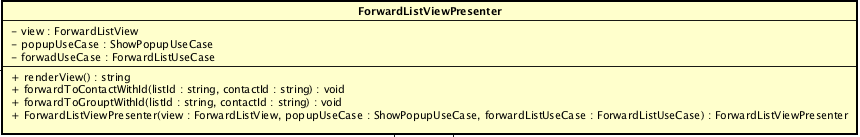
\includegraphics[scale=0.5]{Sezioni/SottosezioniST/img/app/ForwardListViewPresenter.png}
	\caption{feature::forward\_list::presenter::ForwardListViewPresenter}
\end{figure}

\begin{itemize}
\item \textbf{Descrizione}: Questa classe rappresenta il presenter per gli elementi di inoltro della lista-spesa.
\item \textbf{Utilizzo}: Il presenter fa da tramite tra l'implementazione dell'elemento di inoltro e la view, formattando i dati che verranno visualizzati nella view e manipolando gli input dell'utente per eseguire le operazioni predisposte.
\item \textbf{Attributi}: 
	\begin{itemize}
	\item \textit{private chatSource:ChatSource}\\
	La chat sulla quale si vuole intervenire utilizzando questa classe.
	\item \textit{private view:ForwardListView}\\
	La view associata al presenter.
	\item \textit {private forwardListUseCase:ForwardListUseCase}\\
	La componente necessaria alla comunicazione con Rocket.Chat.
	\end{itemize}
\item \textbf{Metodi}:
	\begin{itemize}	
	\item \textit{public ForwardListViewPresenter(view:ForwardListView,popupUseCase:ShowPopupUseCase, forwardListUseCase:ForwardListUseCase):ForwardListViewPresenter}\\
	Il costruttore della classe ForwardListViewPresenter.
	\item{\textbf{Parametri}: \begin{itemize}
			\item \textit{view:ForwardListView}\\
			La view associata al presenter.
			\item \textit{popupUseCase:ShowPopupUseCase}\\
			La chat sulla quale si vuole intervenire utilizzando questa classe.			
			\item \textit{forwardListUseCase:ForwardListUseCase}\\
			La componente necessaria alla comunicazione con Rocket.Chat.
			\end{itemize}}
	\item \textit{public renderView():string}\\
		Genera il codice HTML CSS JS necessario per visualizzare la componente grafica della lista-spesa necessaria alla rimozione di un oggetto da essa.
	\item \textit{public forwardToContactWithId(listId:string,contactId:string):void}\\
	Questo metodo inoltra una particolare lista a un utente Rocket.Chat.
			\item{\textbf{Parametri}: \begin{itemize}
			\item \textit{listId:string}\\
			L'id della lista da inoltrare.
			\item \textit{contactId:string}\\
			L'id dell'utente al quale si vuole inoltrare la lista.
			\end{itemize}}
	\item \textit{public forwardToGroupWithId(listId:string,groupId:string):void}\\
	Questo metodo inoltra una particolare lista a un gruppo in Rocket.Chat.
			\item{\textbf{Parametri}: \begin{itemize}
			\item \textit{listId:string}\\
			L'id della lista da inoltrare.
			\item \textit{groupId:string}\\
			L'id del gruppo al quale si vuole inoltrare la lista.
			\end{itemize}}
	\end{itemize}
\item \textbf{Eventi}:
\end{itemize}

\subsubsection{usecase::ForwardListUseCase}

\label{usecase::ForwardListUseCase}
\begin{figure}[ht]
	\centering
	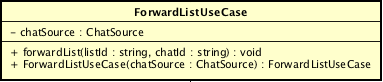
\includegraphics[scale=0.5]{Sezioni/SottosezioniST/img/app/ForwardListUseCase.png}
	\caption{usecase::ForwardListUseCase}
\end{figure}

\begin{itemize}
\item \textbf{Descrizione}: Classe che permette, tramite il contatto diretto con la chat, di inviare la bolla rappresentante la lista ad una specifica chat, eliminandone la parte logica e mantenendone solamente quella grafica, trasformandola in un semplice messaggio di testo
\item \textbf{Utilizzo}: La classe viene utilizzata ogniqualvolta un utente inoltra una lista.
\item \textbf{Attributi}: 
	\begin{itemize}
	\item \textit{private chatSource:ChatSource}\\
	La chat sulla quale la classe opera.
	\end{itemize}
\item \textbf{Metodi}:
	\begin{itemize}
	\item \textit{public forwardList(listId:string, contactId:string):void}\\
	Il metodo inoltra una lista a un particolare contatto.
			\item{\textbf{Parametri}: \begin{itemize}
			\item \textit{listId:string}\\
			L'id della lista da inoltrare.
			\item \textit{contactId:string}\\
			L'id del contatto a cui inoltrare la lista.
			\end{itemize}}
	\item \textit{public ForwardListUseCase(chatSource:ChatSource):ForwardListUseCase}\\
	Il costruttore della classe ForwardListUseCase.
			\item{\textbf{Parametri}: \begin{itemize}
			\item \textit{chatSource:ChatSource}\\
			La chat necessaria alla costruzione di un oggetto di questa classe.
			\end{itemize}}
	\end{itemize}
\item \textbf{Eventi}:
\end{itemize}

\subsubsection{feature::help::HelpView}

\label{feature::help::HelpView}
\begin{figure}[ht]
	\centering
	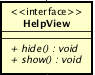
\includegraphics[scale=0.5]{Sezioni/SottosezioniST/img/app/HelpView.png}
	\caption{feature::help::HelpView}
\end{figure}

\begin{itemize}
\item \textbf{Descrizione}: Questa interfaccia rappresenta la view relativa alla richiesta di aiuto da parte di un utente di una lista-spesa.
\item \textbf{Utilizzo}: L'interfaccia viene utilizzata per disaccoppiare presenter e implementazione della richiesta di aiuto, visualizza i dati che gli vengono passati dal presenter.
\item \textbf{Attributi}:
\item \textbf{Metodi}:
	\begin{itemize}
	\item \textit{public hide():void}\\
	Metodo che nasconde la componente grafica necessaria alla richiesta d'aiuto da parte dell'utente.
	\item \textit{public show():void}\\
	Metodo che mostra la componente grafica necessaria alla richiesta d'aiuto da parte dell'utente.
	\end{itemize}
\item \textbf{Eventi}:
\end{itemize}

\subsubsection{feature::help::view::HelpViewImpl}

\label{feature::help::view::HelpViewImpl}
\begin{figure}[ht]
	\centering
	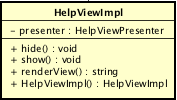
\includegraphics[scale=0.5]{Sezioni/SottosezioniST/img/app/HelpViewImpl.png}
	\caption{feature::help::view::HelpViewImpl}
\end{figure}

\begin{itemize}
\item \textbf{Descrizione}: Questa classe rappresenta la componente grafica necessaria alla richiesta di aiuto di un utente su una lista-spesa, implementando l'interfaccia HelpView.
\item \textbf{Utilizzo}: Questa classe viene utilizzata dall'utente ogniqualvolta richiede aiuto su come usare la lista-spesa.
\item \textbf{Attributi}:
\begin{itemize}
\item \textit{private presenter:HelpViewPresenter}\\
Il presenter associato alla richiesta di aiuto di un utente, al quale questa classe delega la gestione del comportamento dell'elemento di inoltro della lista.
\end{itemize}
\item \textbf{Metodi}:
	\begin{itemize}
	\item \textit{public HelpViewImpl():HelpViewImpl}\\
	Il costruttore della classe HelpViewImpl.
	\item \textit{public hide():void}\\
	Metodo che nasconde la componente grafica necessaria alla richiesta d'aiuto da parte dell'utente.
	\item \textit{public show():void}\\
	Metodo che mostra la componente grafica necessaria alla richiesta d'aiuto da parte dell'utente.
	\item \textit{public renderView():string}\\
	Genera il codice HTML CSS JS necessario per visualizzare la componente grafica della lista-spesa necessaria alla richiesta di aiuto da parte dell'utente.
	\end{itemize}
\item \textbf{Eventi}:
\end{itemize}

\subsubsection{feature::help::presenter::HelpViewPresenter}

\label{feature::help::presenter::HelpViewPresenter}
\begin{figure}[ht]
	\centering
	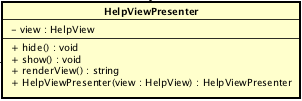
\includegraphics[scale=0.5]{Sezioni/SottosezioniST/img/app/HelpViewPresenter.png}
	\caption{feature::help::presenter::HelpViewPresenter}
\end{figure}

\begin{itemize}
\item \textbf{Descrizione}: Questa classe rappresenta il presenter per gli elementi di richiesta di aiuto della lista-spesa.
\item \textbf{Utilizzo}: Il presenter fa da tramite tra l'implementazione dell'elemento di richiesta di aiuto e la view, formattando i dati che verranno visualizzati nella view e manipolando gli input dell'utente per eseguire le operazioni predisposte.
\item \textbf{Attributi}:
	\begin{itemize}
	\item \textit{private view:HelpView}\\
	La view associata al presenter.
	\end{itemize}
\item \textbf{Metodi}:
	\begin{itemize}
	\item \textit{public HelpViewPresenter(view:HelpView):HelpViewPresenter)}\\
	Il costruttore della classe HelpViewPresenter.
			\item{\textbf{Parametri}: \begin{itemize}
			\item \textit{view:HelpView}\\
			La view necessaria alla costruzione di un oggetto di questa classe.
			\end{itemize}}
	\item \textit{public hide():void}\\
	Metodo che nasconde la componente grafica necessaria alla richiesta d'aiuto da parte dell'utente.
	\item \textit{public show():void}\\
	Metodo che mostra la componente grafica necessaria alla richiesta d'aiuto da parte dell'utente.
	\item \textit{public renderView():string}\\
	Genera il codice HTML CSS JS necessario per visualizzare la componente grafica della lista-spesa necessaria alla richiesta di aiuto da parte dell'utente.
	\end{itemize}
\item \textbf{Eventi}:
\end{itemize}